%=====================================================================
%  Smart Bangladesh Digital City Network -- Design & Implementation
%  CSE421 Computer Networks, BRAC University
%
%  Compile with:  pdflatex SBDC_Report.tex   (run it twice for the ToC)
%
%  EDIT ME: search for  %% EDIT  to find every placeholder.
%=====================================================================
\documentclass[11pt,a4paper]{article}

\usepackage[T1]{fontenc}
\usepackage[utf8]{inputenc}
\usepackage{lmodern}
\usepackage[margin=2.5cm]{geometry}
\usepackage{graphicx}
\usepackage{xcolor}
\usepackage{booktabs}
\usepackage{longtable}
\usepackage{array}
\usepackage{tabularx}
\usepackage{multirow}
\usepackage{listings}
\usepackage{tikz}
\usepackage{enumitem}
\usepackage{fancyhdr}
\usepackage{caption}
\usepackage[hidelinks,bookmarks=true]{hyperref}

%---------------------------------------------------------------- colours
\definecolor{navy}{RGB}{0,60,110}
\definecolor{codebg}{RGB}{246,248,246}
\definecolor{codeframe}{RGB}{200,210,203}
\definecolor{comment}{RGB}{95,120,105}
\definecolor{kw}{RGB}{0,80,140}

%---------------------------------------------------------------- listings
\lstdefinestyle{cisco}{
  basicstyle=\ttfamily\footnotesize,
  backgroundcolor=\color{codebg},
  frame=single,
  rulecolor=\color{codeframe},
  framesep=5pt,
  breaklines=true,
  breakatwhitespace=true,
  columns=fullflexible,
  keepspaces=true,
  showstringspaces=false,
  morecomment=[l]{!},
  commentstyle=\color{comment}\itshape,
  keywordstyle=\color{kw}\bfseries,
  morekeywords={hostname,interface,router,rip,version,network,dhcp,pool,
    excluded-address,default-router,dns-server,domain-name,helper-address,
    passive-interface,redistribute,static,metric,timers,basic,clock,rate,
    shutdown,auto-summary,description,enable,secret,banner,motd,line,console,
    vty,password,login,logging,synchronous,configure,terminal,end,exit,copy,
    running-config,startup-config,show,ping,tracert,route},
  captionpos=b,
  aboveskip=8pt,
  belowskip=8pt
}
\lstset{style=cisco}

%---------------------------------------------------------------- headers
\pagestyle{fancy}
\fancyhf{}
\fancyhead[L]{\small\itshape Smart Bangladesh Digital City Network}
\fancyhead[R]{\small CSE421}
\fancyfoot[C]{\small\thepage}
\renewcommand{\headrulewidth}{0.4pt}

\setlist{itemsep=2pt,parsep=0pt,topsep=4pt}
\captionsetup{font=small,labelfont={bf,color=navy}}
\renewcommand{\arraystretch}{1.15}

%---------------------------------------------------------------- helpers
\newcommand{\netc}[1]{\texttt{\small #1}}
\newcommand{\tnode}[3]{\node[anchor=west,font=\small\ttfamily] at (#1,#2) {#3};}
\newcommand{\tdesc}[3]{\node[anchor=west,font=\small] at (#1,#2) {#3};}

%=====================================================================
\begin{document}

%---------------------------------------------------------------- COVER
\begin{titlepage}
\centering
\vspace*{6mm}

% %% EDIT: uncomment and supply a logo file if your group uses one
% \includegraphics[width=0.28\textwidth]{bracu_logo.png}\\[10mm]

{\LARGE\scshape BRAC University\par}
\vspace{5mm}
{\large Department of Computer Science and Engineering\par}

\vspace{26mm}
{\color{navy}\rule{\linewidth}{1.2pt}}
\vspace{8mm}

{\huge\bfseries Smart Bangladesh Digital City Network\par}
\vspace{6mm}
{\Large Design and Implementation Report\par}

\vspace{8mm}
{\color{navy}\rule{\linewidth}{1.2pt}}

\vspace{20mm}
{\large \textbf{Course Code:} CSE421 \par}
\vspace{3mm}
{\large \textbf{Course Name:} Computer Networks \par}
\vspace{3mm}
{\large \textbf{Group Number:} Group 01 \par}

\vspace{18mm}
{\large\bfseries Submitted by\par}
\vspace{5mm}

% %% EDIT: replace the two placeholder rows with the real names and IDs
\begin{tabular}{@{}p{75mm}p{35mm}@{}}
\toprule
\textbf{Name} & \textbf{Student ID} \\
\midrule
Mohammad Jabir Safa Khandoker   & 22201108 \\
Md. Saadat Rahman   & 22201101 \\
Nazah S. Anis & 22201105 \\
\bottomrule
\end{tabular}

\vfill
{\large August 2026\par}
\vspace{4mm}
\end{titlepage}

%---------------------------------------------------------------- ToC
\pagenumbering{roman}
\setcounter{page}{1}
\tableofcontents
\clearpage
\listoftables
\clearpage
\pagenumbering{arabic}
\setcounter{page}{1}

%=====================================================================

\section{Assumptions and Design Decisions}
\label{sec:assumptions}

The specification leaves several points open. Each decision below is stated
together with the reason it was taken, so that the design can be assessed on
its reasoning and not only on its output.

\subsection{A1 --- The PHD--TMA link is excluded from RIP}
The specification requires a direct PHD--TMA link and also requires that a failure of the SCCC--TMA path reroute traffic through
TMA $\rightarrow$ DCS $\rightarrow$ ERU $\rightarrow$ SCCC. These two clauses conflict. If RIP runs across the PHD--TMA serial, then when TMA loses the central switch it simply relearns every network from PHD at administrative distance 120, the floating static at distance 130 never installs, and the required backup path is never taken.

The link is therefore cabled, addressed and reachable, but is declared
\netc{passive-interface} in RIP on \emph{both} routers. Its subnet is still advertised to the rest of the network, while no routing information crosses it. The physical redundancy the brief asks for exists, and the failover path remains deterministic.

\subsection{A2 --- SCCC redistributes its static routes into RIP}
SCCC is required to run both dynamic and static routing and to know every network. On its own this does not let TMA and PHD, which are RIP-only, learn the ERU, DCS and ESC networks. The command \netc{redistribute static metric 5} under \netc{router rip} on SCCC is what makes the requirement that TMA reach all external networks through SCCC true in practice.

\subsection{A3 --- DNS, and the absence of MX records in Packet Tracer}
A single DNS server at SCCC is authoritative for all zones and is handed to every host by DHCP. Packet Tracer implements no MX record type; when a mail server relays a message addressed to another domain it performs a plain A lookup on the bare domain name. Records for \netc{tma.gov.bd} and \netc{esc.gov.bd} are therefore published in addition to the \netc{mail.*} names, and both mail servers are configured with \netc{11.8.1.250} as their own DNS server. Without this, mail inside each domain works and cross-domain mail fails.

\subsection{A4 --- Address reservation convention}
In every LAN, host addresses \netc{.1} to \netc{.9} are reserved for the
gateway and future infrastructure, and the top of the range is reserved for
servers and printers. Both bands are excluded from the DHCP pools, so a
dynamically assigned address can never collide with a static one.

\subsection{A5 --- Laboratory credentials}
All routers use \netc{enable secret cisco123} and line password \netc{cisco};
all mail accounts use password \netc{cisco123}.

\clearpage
%=====================================================================
\section{VLSM Design}

\subsection{Base network}
Student ID \netc{22201108} $\rightarrow$ last four digits \netc{1108}
$\rightarrow$ pairs \netc{11} and \netc{08} $\rightarrow$ base network
\netc{11.8.0.0/16}, mask \netc{255.255.0.0}, giving 65\,536 addresses.

\subsection{Sizing the subnets}
Each requirement is rounded up to the next power of two after adding two
addresses for the network and broadcast addresses. Blocks are then allocated
largest-first, so that a small subnet can never block a large one.
Table~\ref{tab:sizing} shows the calculation.

\begin{table}[htbp]
\centering
\caption{Host requirement to block size}
\label{tab:sizing}
\small
\begin{tabular}{@{}clrrrcrr@{}}
\toprule
\textbf{Order} & \textbf{Network} & \textbf{Hosts} & \textbf{+2} & \textbf{Block} & \textbf{Prefix} & \textbf{Usable} & \textbf{Spare} \\
\midrule
1     & SCCC LAN            & 320 & 322 & 512 & /23 & 510 & 190 \\
2     & DCS LAN             & 260 & 262 & 512 & /23 & 510 & 250 \\
3     & PHD LAN             & 220 & 222 & 256 & /24 & 254 & 34 \\
4     & TMA LAN             & 180 & 182 & 256 & /24 & 254 & 74 \\
5     & ESC LAN             & 140 & 142 & 256 & /24 & 254 & 114 \\
6     & ERU LAN             & 100 & 102 & 128 & /25 & 126 & 26 \\
7     & Central segment     & 3   & 5   & 8   & /29 & 6   & 3 \\
8--12 & WAN links (5 of)    & 2   & 4   & 4   & /30 & 2   & 0 \\
\bottomrule
\end{tabular}
\end{table}

\noindent

\subsection{VLSM allocation tree}

Figure~\ref{fig:tree1} shows how \netc{11.8.0.0/16} is divided down to the six
department LANs. The whole design fits inside \netc{11.8.0.0/21}; everything
from \netc{11.8.8.0} upward is left untouched for growth.
Figure~\ref{fig:tree2} expands the infrastructure block.

\begin{figure}[htbp]
\centering
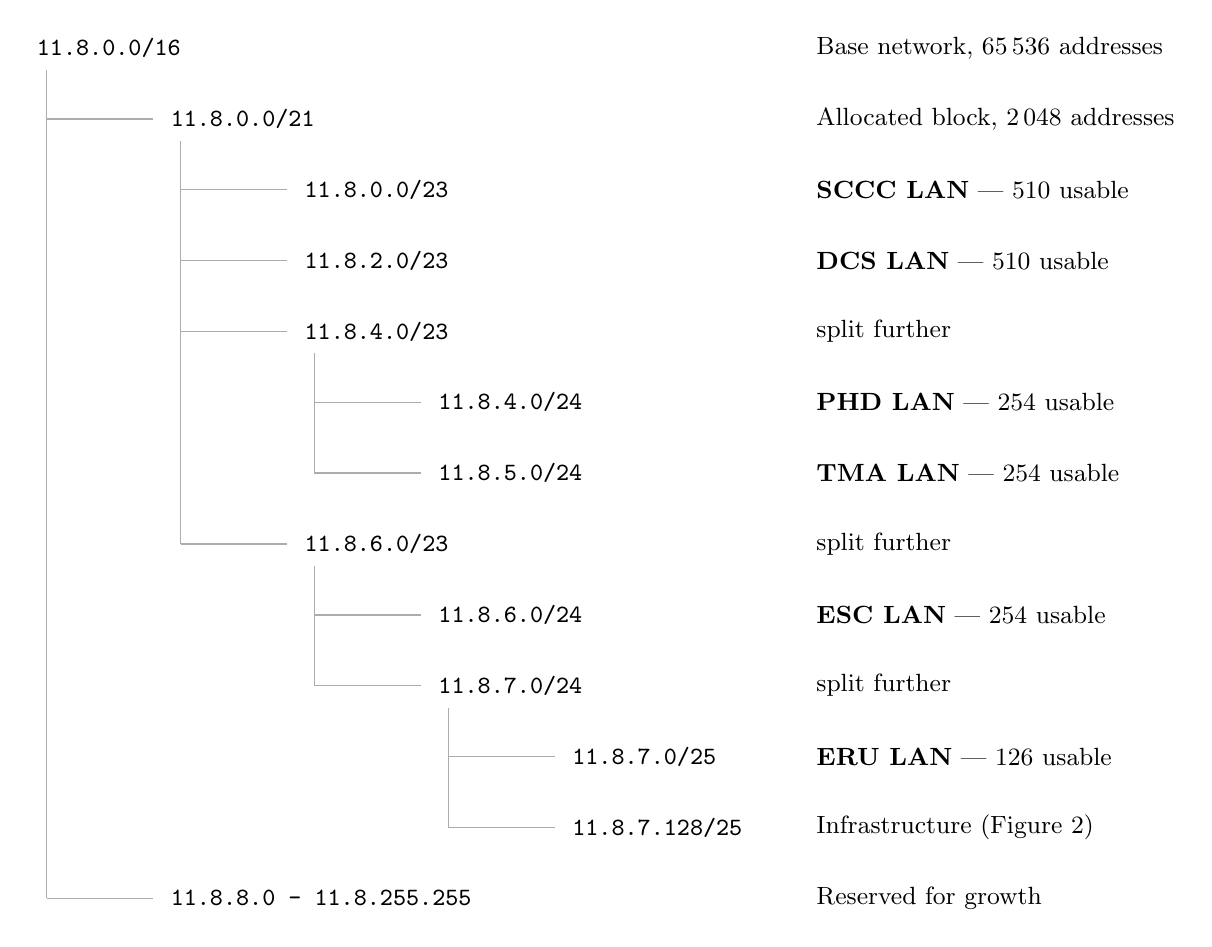
\begin{tikzpicture}[line width=0.5pt]
% ---- connector lines
\draw[gray!65] (0.25,-0.28) -- (0.25,-10.8);
\draw[gray!65] (0.25,-0.9)  -- (1.60,-0.9);
\draw[gray!65] (0.25,-10.8) -- (1.60,-10.8);

\draw[gray!65] (1.95,-1.18) -- (1.95,-6.3);
\draw[gray!65] (1.95,-1.8)  -- (3.30,-1.8);
\draw[gray!65] (1.95,-2.7)  -- (3.30,-2.7);
\draw[gray!65] (1.95,-3.6)  -- (3.30,-3.6);
\draw[gray!65] (1.95,-6.3)  -- (3.30,-6.3);

\draw[gray!65] (3.65,-3.88) -- (3.65,-5.4);
\draw[gray!65] (3.65,-4.5)  -- (5.00,-4.5);
\draw[gray!65] (3.65,-5.4)  -- (5.00,-5.4);

\draw[gray!65] (3.65,-6.58) -- (3.65,-8.1);
\draw[gray!65] (3.65,-7.2)  -- (5.00,-7.2);
\draw[gray!65] (3.65,-8.1)  -- (5.00,-8.1);

\draw[gray!65] (5.35,-8.38) -- (5.35,-9.9);
\draw[gray!65] (5.35,-9.0)  -- (6.70,-9.0);
\draw[gray!65] (5.35,-9.9)  -- (6.70,-9.9);

% ---- subnet labels
\tnode{0.0}{0.0}{\textbf{11.8.0.0/16}}
\tnode{1.7}{-0.9}{11.8.0.0/21}
\tnode{3.4}{-1.8}{11.8.0.0/23}
\tnode{3.4}{-2.7}{11.8.2.0/23}
\tnode{3.4}{-3.6}{11.8.4.0/23}
\tnode{5.1}{-4.5}{11.8.4.0/24}
\tnode{5.1}{-5.4}{11.8.5.0/24}
\tnode{3.4}{-6.3}{11.8.6.0/23}
\tnode{5.1}{-7.2}{11.8.6.0/24}
\tnode{5.1}{-8.1}{11.8.7.0/24}
\tnode{6.8}{-9.0}{11.8.7.0/25}
\tnode{6.8}{-9.9}{11.8.7.128/25}
\tnode{1.7}{-10.8}{11.8.8.0 - 11.8.255.255}

% ---- descriptions
\tdesc{9.9}{0.0}{Base network, 65\,536 addresses}
\tdesc{9.9}{-0.9}{Allocated block, 2\,048 addresses}
\tdesc{9.9}{-1.8}{\textbf{SCCC LAN} --- 510 usable}
\tdesc{9.9}{-2.7}{\textbf{DCS LAN} --- 510 usable}
\tdesc{9.9}{-3.6}{split further}
\tdesc{9.9}{-4.5}{\textbf{PHD LAN} --- 254 usable}
\tdesc{9.9}{-5.4}{\textbf{TMA LAN} --- 254 usable}
\tdesc{9.9}{-6.3}{split further}
\tdesc{9.9}{-7.2}{\textbf{ESC LAN} --- 254 usable}
\tdesc{9.9}{-8.1}{split further}
\tdesc{9.9}{-9.0}{\textbf{ERU LAN} --- 126 usable}
\tdesc{9.9}{-9.9}{Infrastructure (Figure 2)}
\tdesc{9.9}{-10.8}{Reserved for growth}
\end{tikzpicture}
\caption{VLSM allocation tree for the six department LANs}
\label{fig:tree1}
\end{figure}

\begin{figure}[htbp]
\centering
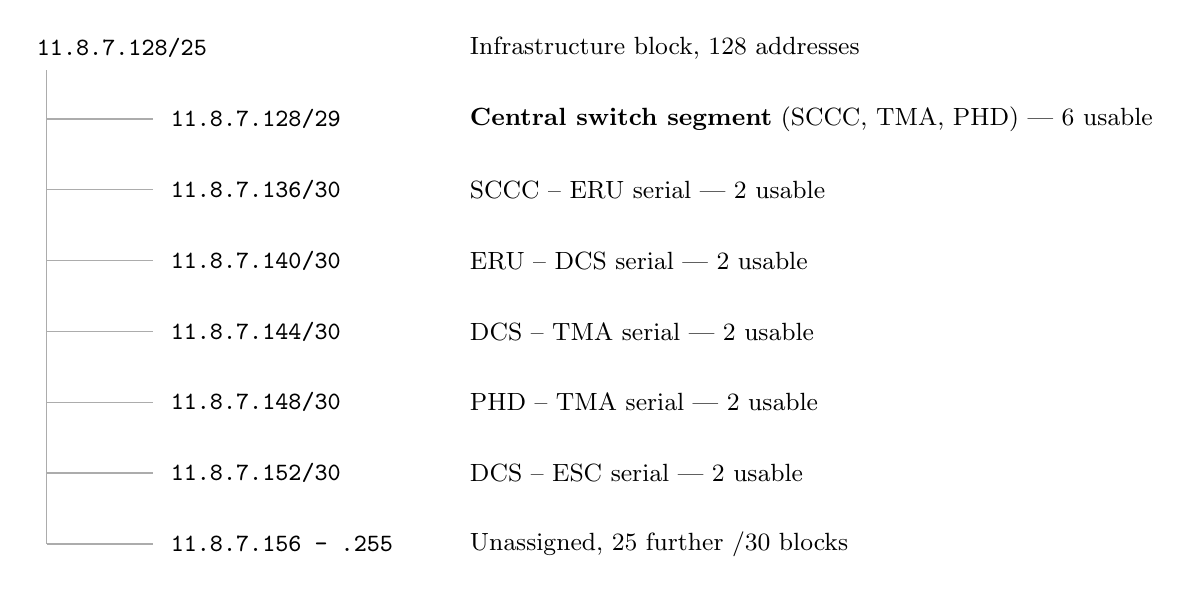
\begin{tikzpicture}[line width=0.5pt]
\draw[gray!65] (0.25,-0.28) -- (0.25,-6.3);
\foreach \y in {-0.9,-1.8,-2.7,-3.6,-4.5,-5.4,-6.3}
  { \draw[gray!65] (0.25,\y) -- (1.60,\y); }

\tnode{0.0}{0.0}{\textbf{11.8.7.128/25}}
\tnode{1.7}{-0.9}{11.8.7.128/29}
\tnode{1.7}{-1.8}{11.8.7.136/30}
\tnode{1.7}{-2.7}{11.8.7.140/30}
\tnode{1.7}{-3.6}{11.8.7.144/30}
\tnode{1.7}{-4.5}{11.8.7.148/30}
\tnode{1.7}{-5.4}{11.8.7.152/30}
\tnode{1.7}{-6.3}{11.8.7.156 - .255}

\tdesc{5.5}{0.0}{Infrastructure block, 128 addresses}
\tdesc{5.5}{-0.9}{\textbf{Central switch segment} (SCCC, TMA, PHD) --- 6 usable}
\tdesc{5.5}{-1.8}{SCCC -- ERU serial --- 2 usable}
\tdesc{5.5}{-2.7}{ERU -- DCS serial --- 2 usable}
\tdesc{5.5}{-3.6}{DCS -- TMA serial --- 2 usable}
\tdesc{5.5}{-4.5}{PHD -- TMA serial --- 2 usable}
\tdesc{5.5}{-5.4}{DCS -- ESC serial --- 2 usable}
\tdesc{5.5}{-6.3}{Unassigned, 25 further /30 blocks}
\end{tikzpicture}
\caption{Expansion of the infrastructure block \texttt{11.8.7.128/25}}
\label{fig:tree2}
\end{figure}

\subsection{Subnet summary}

\begin{table}[htbp]
\centering
\caption{Complete VLSM allocation from 11.8.0.0/16}
\label{tab:vlsm}
\small
\begin{tabular}{@{}lllllc@{}}
\toprule
\textbf{Subnet} & \textbf{Network} & \textbf{Mask} &
\textbf{First host} & \textbf{Last host} & \textbf{Broadcast} \\
\midrule
SCCC LAN        & 11.8.0.0/23    & 255.255.254.0   & 11.8.0.1   & 11.8.1.254 & 11.8.1.255 \\
DCS LAN         & 11.8.2.0/23    & 255.255.254.0   & 11.8.2.1   & 11.8.3.254 & 11.8.3.255 \\
PHD LAN         & 11.8.4.0/24    & 255.255.255.0   & 11.8.4.1   & 11.8.4.254 & 11.8.4.255 \\
TMA LAN         & 11.8.5.0/24    & 255.255.255.0   & 11.8.5.1   & 11.8.5.254 & 11.8.5.255 \\
ESC LAN         & 11.8.6.0/24    & 255.255.255.0   & 11.8.6.1   & 11.8.6.254 & 11.8.6.255 \\
ERU LAN         & 11.8.7.0/25    & 255.255.255.128 & 11.8.7.1   & 11.8.7.126 & 11.8.7.127 \\
Central segment & 11.8.7.128/29  & 255.255.255.248 & 11.8.7.129 & 11.8.7.134 & 11.8.7.135 \\
SCCC -- ERU     & 11.8.7.136/30  & 255.255.255.252 & 11.8.7.137 & 11.8.7.138 & 11.8.7.139 \\
ERU -- DCS      & 11.8.7.140/30  & 255.255.255.252 & 11.8.7.141 & 11.8.7.142 & 11.8.7.143 \\
DCS -- TMA      & 11.8.7.144/30  & 255.255.255.252 & 11.8.7.145 & 11.8.7.146 & 11.8.7.147 \\
PHD -- TMA      & 11.8.7.148/30  & 255.255.255.252 & 11.8.7.149 & 11.8.7.150 & 11.8.7.151 \\
DCS -- ESC      & 11.8.7.152/30  & 255.255.255.252 & 11.8.7.153 & 11.8.7.154 & 11.8.7.155 \\
\bottomrule
\end{tabular}
\end{table}

\clearpage
%=====================================================================
\section{IP Addressing Table}

Routers, printers and servers use static addresses; all PCs receive their
addresses dynamically. Every static host sits at the top of its LAN range and
is excluded from the corresponding DHCP pool.

\subsection{Router interfaces}

\begin{longtable}{@{}p{20mm}p{22mm}p{34mm}p{26mm}p{30mm}@{}}
\caption{Router interface addressing}\label{tab:routers}\\
\toprule
\textbf{Router} & \textbf{Interface} & \textbf{Connects to} &
\textbf{IP address} & \textbf{Mask} \\
\midrule
\endfirsthead
\multicolumn{5}{@{}l}{\small\itshape Table \thetable\ continued from previous page}\\
\toprule
\textbf{Router} & \textbf{Interface} & \textbf{Connects to} &
\textbf{IP address} & \textbf{Mask} \\
\midrule
\endhead
\bottomrule
\endfoot
R-SCCC & Fa0/0   & SCCC LAN switch  & 11.8.0.1   & 255.255.254.0 \\
R-SCCC & Fa0/1   & Central switch   & 11.8.7.129 & 255.255.255.248 \\
R-SCCC & Se0/0/0 & R-ERU Se0/0/0    & 11.8.7.137 & 255.255.255.252 \\
\midrule
R-TMA  & Fa0/0   & TMA LAN switch   & 11.8.5.1   & 255.255.255.0 \\
R-TMA  & Fa0/1   & Central switch   & 11.8.7.130 & 255.255.255.248 \\
R-TMA  & Se0/0/0 & R-DCS Se0/0/0    & 11.8.7.146 & 255.255.255.252 \\
R-TMA  & Se0/0/1 & R-PHD Se0/0/0    & 11.8.7.149 & 255.255.255.252 \\
\midrule
R-PHD  & Fa0/0   & PHD LAN switch   & 11.8.4.1   & 255.255.255.0 \\
R-PHD  & Fa0/1   & Central switch   & 11.8.7.131 & 255.255.255.248 \\
R-PHD  & Se0/0/0 & R-TMA Se0/0/1    & 11.8.7.150 & 255.255.255.252 \\
\midrule
R-ERU  & Fa0/0   & ERU LAN switch   & 11.8.7.1   & 255.255.255.128 \\
R-ERU  & Se0/0/0 & R-SCCC Se0/0/0   & 11.8.7.138 & 255.255.255.252 \\
R-ERU  & Se0/0/1 & R-DCS Se0/1/0    & 11.8.7.141 & 255.255.255.252 \\
\midrule
R-DCS  & Fa0/0   & DCS LAN switch   & 11.8.2.1   & 255.255.254.0 \\
R-DCS  & Se0/0/0 & R-TMA Se0/0/0    & 11.8.7.145 & 255.255.255.252 \\
R-DCS  & Se0/0/1 & R-ESC Se0/0/0    & 11.8.7.153 & 255.255.255.252 \\
R-DCS  & Se0/1/0 & R-ERU Se0/0/1    & 11.8.7.142 & 255.255.255.252 \\
\midrule
R-ESC  & Fa0/0   & ESC LAN switch   & 11.8.6.1   & 255.255.255.0 \\
R-ESC  & Se0/0/0 & R-DCS Se0/0/1    & 11.8.7.154 & 255.255.255.252 \\
\end{longtable}

\noindent
Exactly one end of each serial link is the DCE and carries
\netc{clock rate 64000}. The five DCE ends are
R-SCCC Se0/0/0, R-TMA Se0/0/1, R-ERU Se0/0/1, R-DCS Se0/0/0 and
R-DCS Se0/0/1.

\subsection{Servers and printers}

\begin{longtable}{@{}p{16mm}p{30mm}p{42mm}p{24mm}p{24mm}@{}}
\caption{Static addressing for servers and printers}\label{tab:servers}\\
\toprule
\textbf{Dept.} & \textbf{Device} & \textbf{Role} &
\textbf{IP address} & \textbf{Gateway} \\
\midrule
\endfirsthead
\toprule
\textbf{Dept.} & \textbf{Device} & \textbf{Role} &
\textbf{IP address} & \textbf{Gateway} \\
\midrule
\endhead
\bottomrule
\endfoot
SCCC & SRV-DNS       & Central DNS server        & 11.8.1.250 & 11.8.0.1 \\
SCCC & SRV-WEB-SC    & www.smartcity.gov.bd      & 11.8.1.251 & 11.8.0.1 \\
SCCC & PRN-SCCC      & Network printer           & 11.8.1.254 & 11.8.0.1 \\
\midrule
DCS  & SRV-DHCP-DCS  & DHCP for DCS and ESC      & 11.8.2.250 & 11.8.2.1 \\
DCS  & PRN-DCS       & Network printer           & 11.8.3.254 & 11.8.2.1 \\
\midrule
PHD  & PRN-PHD       & Network printer           & 11.8.4.254 & 11.8.4.1 \\
\midrule
TMA  & SRV-MAIL-TMA  & mail.tma.gov.bd           & 11.8.5.250 & 11.8.5.1 \\
TMA  & PRN-TMA       & Network printer           & 11.8.5.254 & 11.8.5.1 \\
\midrule
ESC  & SRV-MAIL-ESC  & mail.esc.gov.bd           & 11.8.6.250 & 11.8.6.1 \\
ESC  & PRN-ESC       & Network printer           & 11.8.6.254 & 11.8.6.1 \\
\midrule
ERU  & SRV-WEB-ER    & www.emergency.gov.bd      & 11.8.7.120 & 11.8.7.1 \\
ERU  & SRV-DHCP-ERU  & DHCP for ERU              & 11.8.7.121 & 11.8.7.1 \\
ERU  & PRN-ERU       & Network printer           & 11.8.7.126 & 11.8.7.1 \\
\end{longtable}

\noindent
Every device in Table~\ref{tab:servers} uses \netc{11.8.1.250} as its DNS
server, including the two mail servers, which need it in order to relay
cross-domain messages.

\subsection{DHCP pools}

\begin{table}[htbp]
\centering
\caption{Dynamic address ranges}
\label{tab:dhcp}
\small
\begin{tabular}{@{}llllc@{}}
\toprule
\textbf{LAN} & \textbf{Served by} & \textbf{Pool range} &
\textbf{Gateway} & \textbf{Delivery} \\
\midrule
SCCC & R-SCCC, pool SCCC-POOL & 11.8.0.10 -- 11.8.1.199 & 11.8.0.1 & direct \\
TMA  & R-SCCC, pool TMA-POOL  & 11.8.5.10 -- 11.8.5.199 & 11.8.5.1 & relay \\
PHD  & R-SCCC, pool PHD-POOL  & 11.8.4.10 -- 11.8.4.199 & 11.8.4.1 & relay \\
DCS  & SRV-DHCP-DCS           & 11.8.2.10 -- 11.8.3.199 & 11.8.2.1 & direct \\
ESC  & SRV-DHCP-DCS           & 11.8.6.10 -- 11.8.6.199 & 11.8.6.1 & relay \\
ERU  & SRV-DHCP-ERU           & 11.8.7.10 -- 11.8.7.99  & 11.8.7.1 & direct \\
\bottomrule
\end{tabular}
\end{table}

\noindent
All six pools hand out \netc{11.8.1.250} as the DNS server. The relayed pools
are reached through \netc{ip helper-address}: TMA and PHD point at
\netc{11.8.7.129} (the SCCC router), and ESC points at \netc{11.8.2.250}
(the DCS server).

\clearpage
%=====================================================================
\section{Configuration Commands}

Every block below begins from user EXEC mode and assumes \netc{enable}
followed by \netc{configure terminal}. Each router is finished with
\netc{end} and \netc{copy running-config startup-config}.

\subsection{R-SCCC}

\begin{lstlisting}
hostname R-SCCC
no ip domain-lookup
enable secret cisco123
banner motd #SBDC - Smart City Control Center - Authorized access only#
line console 0
 password cisco
 login
 logging synchronous
line vty 0 4
 password cisco
 login
exit
!--- interfaces
interface FastEthernet0/0
 description SCCC LAN
 ip address 11.8.0.1 255.255.254.0
 no shutdown
interface FastEthernet0/1
 description Central switch segment
 ip address 11.8.7.129 255.255.255.248
 no shutdown
interface Serial0/0/0
 description Serial to R-ERU DCE side
 ip address 11.8.7.137 255.255.255.252
 clock rate 64000
 no shutdown
exit
!--- DHCP server for SCCC, TMA and PHD
ip dhcp excluded-address 11.8.0.1 11.8.0.9
ip dhcp excluded-address 11.8.1.200 11.8.1.254
ip dhcp excluded-address 11.8.5.1 11.8.5.9
ip dhcp excluded-address 11.8.5.200 11.8.5.254
ip dhcp excluded-address 11.8.4.1 11.8.4.9
ip dhcp excluded-address 11.8.4.200 11.8.4.254
ip dhcp pool SCCC-POOL
 network 11.8.0.0 255.255.254.0
 default-router 11.8.0.1
 dns-server 11.8.1.250
 domain-name smartcity.gov.bd
ip dhcp pool TMA-POOL
 network 11.8.5.0 255.255.255.0
 default-router 11.8.5.1
 dns-server 11.8.1.250
ip dhcp pool PHD-POOL
 network 11.8.4.0 255.255.255.0
 default-router 11.8.4.1
 dns-server 11.8.1.250
exit
!--- dynamic routing
router rip
 version 2
 no auto-summary
 network 11.0.0.0
 passive-interface FastEthernet0/0
 passive-interface Serial0/0/0
 timers basic 10 30 30 40
 redistribute static metric 5
exit
!--- static routes toward the ERU / DCS / ESC side
ip route 11.8.7.0   255.255.255.128 11.8.7.138
ip route 11.8.7.140 255.255.255.252 11.8.7.138
ip route 11.8.2.0   255.255.254.0   11.8.7.138
ip route 11.8.7.144 255.255.255.252 11.8.7.138
ip route 11.8.7.152 255.255.255.252 11.8.7.138
ip route 11.8.6.0   255.255.255.0   11.8.7.138
!--- floating backup to the TMA LAN, distance 130
ip route 11.8.5.0   255.255.255.0   11.8.7.138 130
\end{lstlisting}

\subsection{R-TMA}

\begin{lstlisting}
hostname R-TMA
no ip domain-lookup
enable secret cisco123
banner motd #SBDC - Traffic Management Authority#
line console 0
 password cisco
 login
 logging synchronous
line vty 0 4
 password cisco
 login
exit
interface FastEthernet0/0
 description TMA LAN
 ip address 11.8.5.1 255.255.255.0
 ip helper-address 11.8.7.129
 no shutdown
interface FastEthernet0/1
 description Central switch - PRIMARY PATH, failed during the demo
 ip address 11.8.7.130 255.255.255.248
 no shutdown
interface Serial0/0/0
 description Serial to R-DCS - backup path
 ip address 11.8.7.146 255.255.255.252
 no shutdown
interface Serial0/0/1
 description Serial to R-PHD DCE side - physical redundancy only
 ip address 11.8.7.149 255.255.255.252
 clock rate 64000
 no shutdown
exit
router rip
 version 2
 no auto-summary
 network 11.0.0.0
 passive-interface FastEthernet0/0
 passive-interface Serial0/0/0
 passive-interface Serial0/0/1
 timers basic 10 30 30 40
exit
!--- floating static routes via DCS, administrative distance 130
ip route 11.8.0.0   255.255.254.0   11.8.7.145 130
ip route 11.8.4.0   255.255.255.0   11.8.7.145 130
ip route 11.8.2.0   255.255.254.0   11.8.7.145 130
ip route 11.8.6.0   255.255.255.0   11.8.7.145 130
ip route 11.8.7.0   255.255.255.128 11.8.7.145 130
ip route 11.8.7.128 255.255.255.248 11.8.7.145 130
ip route 11.8.7.136 255.255.255.252 11.8.7.145 130
ip route 11.8.7.140 255.255.255.252 11.8.7.145 130
ip route 11.8.7.152 255.255.255.252 11.8.7.145 130
\end{lstlisting}

\subsection{R-PHD}

\begin{lstlisting}
hostname R-PHD
no ip domain-lookup
enable secret cisco123
banner motd #SBDC - Public Health Department#
line console 0
 password cisco
 login
 logging synchronous
line vty 0 4
 password cisco
 login
exit
interface FastEthernet0/0
 description PHD LAN
 ip address 11.8.4.1 255.255.255.0
 ip helper-address 11.8.7.129
 no shutdown
interface FastEthernet0/1
 description Central switch segment
 ip address 11.8.7.131 255.255.255.248
 no shutdown
interface Serial0/0/0
 description Serial to R-TMA - physical redundancy only
 ip address 11.8.7.150 255.255.255.252
 no shutdown
exit
router rip
 version 2
 no auto-summary
 network 11.0.0.0
 passive-interface FastEthernet0/0
 passive-interface Serial0/0/0
 timers basic 10 30 30 40
\end{lstlisting}

\subsection{R-ERU}

\begin{lstlisting}
hostname R-ERU
no ip domain-lookup
enable secret cisco123
banner motd #SBDC - Emergency Response Unit#
line console 0
 password cisco
 login
 logging synchronous
line vty 0 4
 password cisco
 login
exit
interface FastEthernet0/0
 description ERU LAN
 ip address 11.8.7.1 255.255.255.128
 no shutdown
interface Serial0/0/0
 description Serial to R-SCCC
 ip address 11.8.7.138 255.255.255.252
 no shutdown
interface Serial0/0/1
 description Serial to R-DCS DCE side
 ip address 11.8.7.141 255.255.255.252
 clock rate 64000
 no shutdown
exit
!--- reached through SCCC
ip route 11.8.0.0   255.255.254.0   11.8.7.137
ip route 11.8.4.0   255.255.255.0   11.8.7.137
ip route 11.8.7.128 255.255.255.248 11.8.7.137
ip route 11.8.7.148 255.255.255.252 11.8.7.137
!--- reached through DCS
ip route 11.8.2.0   255.255.254.0   11.8.7.142
ip route 11.8.6.0   255.255.255.0   11.8.7.142
ip route 11.8.5.0   255.255.255.0   11.8.7.142
ip route 11.8.7.144 255.255.255.252 11.8.7.142
ip route 11.8.7.152 255.255.255.252 11.8.7.142
\end{lstlisting}

\subsection{R-DCS}

\begin{lstlisting}
hostname R-DCS
no ip domain-lookup
enable secret cisco123
banner motd #SBDC - Digital Citizen Service#
line console 0
 password cisco
 login
 logging synchronous
line vty 0 4
 password cisco
 login
exit
interface FastEthernet0/0
 description DCS LAN
 ip address 11.8.2.1 255.255.254.0
 no shutdown
interface Serial0/0/0
 description Serial to R-TMA DCE side
 ip address 11.8.7.145 255.255.255.252
 clock rate 64000
 no shutdown
interface Serial0/0/1
 description Serial to R-ESC DCE side
 ip address 11.8.7.153 255.255.255.252
 clock rate 64000
 no shutdown
interface Serial0/1/0
 description Serial to R-ERU
 ip address 11.8.7.142 255.255.255.252
 no shutdown
exit
!--- out of Serial0/0/0, toward TMA
ip route 11.8.5.0   255.255.255.0   Serial0/0/0
ip route 11.8.7.148 255.255.255.252 Serial0/0/0
!--- out of Serial0/0/1, toward ESC
ip route 11.8.6.0   255.255.255.0   Serial0/0/1
!--- out of Serial0/1/0, toward ERU and everything beyond it
ip route 11.8.0.0   255.255.254.0   Serial0/1/0
ip route 11.8.4.0   255.255.255.0   Serial0/1/0
ip route 11.8.7.0   255.255.255.128 Serial0/1/0
ip route 11.8.7.128 255.255.255.248 Serial0/1/0
ip route 11.8.7.136 255.255.255.252 Serial0/1/0
\end{lstlisting}

\subsection{R-ESC}

\begin{lstlisting}
hostname R-ESC
no ip domain-lookup
enable secret cisco123
banner motd #SBDC - Education Service Center#
line console 0
 password cisco
 login
 logging synchronous
line vty 0 4
 password cisco
 login
exit
interface FastEthernet0/0
 description ESC LAN
 ip address 11.8.6.1 255.255.255.0
 ip helper-address 11.8.2.250
 no shutdown
interface Serial0/0/0
 description Serial to R-DCS
 ip address 11.8.7.154 255.255.255.252
 no shutdown
exit
!--- exactly one route, and nothing else
ip route 0.0.0.0 0.0.0.0 11.8.7.153
\end{lstlisting}

\clearpage
%=====================================================================
\section{Server Configuration}

The seven servers are configured through the Packet Tracer GUI rather than a
CLI. The settings applied are recorded below.

\subsection{DNS Server}

Services $\rightarrow$ DNS $\rightarrow$ On, then add each record and press
\textbf{Add}.

\begin{table}[htbp]
\centering
\caption{DNS zone records}
\label{tab:dns}
\small
\begin{tabular}{@{}llll@{}}
\toprule
\textbf{Name} & \textbf{Type} & \textbf{Address} & \textbf{Purpose} \\
\midrule
www.smartcity.gov.bd  & A & 11.8.1.251 & SCCC website \\
www.emergency.gov.bd  & A & 11.8.7.120 & ERU website \\
mail.tma.gov.bd       & A & 11.8.5.250 & TMA mail client server field \\
mail.esc.gov.bd       & A & 11.8.6.250 & ESC mail client server field \\
tma.gov.bd            & A & 11.8.5.250 & cross-domain SMTP relay \\
esc.gov.bd            & A & 11.8.6.250 & cross-domain SMTP relay \\
smartcity.gov.bd      & A & 11.8.1.251 & convenience \\
emergency.gov.bd      & A & 11.8.7.120 & convenience \\
\bottomrule
\end{tabular}
\end{table}

\noindent

\subsection{Web Servers}

On SRV-WEB-SC and SRV-WEB-ER: Services $\rightarrow$ HTTP $\rightarrow$ On,
then edit \netc{index.html}.

\begin{lstlisting}[morecomment={[s]{<!--}{-->}}]
<!-- SRV-WEB-SC : www.smartcity.gov.bd -->
<html><body>
<h1>Smart City Control Center</h1>
<p>Smart Bangladesh Digital City - central services portal.</p>
<p>Server 11.8.1.251 - SCCC LAN 11.8.0.0/23</p>
</body></html>

<!-- SRV-WEB-ER : www.emergency.gov.bd -->
<html><body>
<h1>Emergency Response Unit</h1>
<p>24/7 emergency coordination - Smart Bangladesh Digital City.</p>
<p>Server 11.8.7.120 - ERU LAN 11.8.7.0/25</p>
</body></html>
\end{lstlisting}

\subsection{DHCP Servers}

Services $\rightarrow$ DHCP $\rightarrow$ On, fill the pool, then press
\textbf{Add}.

\begin{table}[htbp]
\centering
\caption{Server-based DHCP pools}
\label{tab:dhcpsrv}
\small
\begin{tabular}{@{}lllllr@{}}
\toprule
\textbf{Server} & \textbf{Pool} & \textbf{Gateway} & \textbf{Start IP} &
\textbf{Mask} & \textbf{Max} \\
\midrule
SRV-DHCP-DCS & DCS-POOL & 11.8.2.1 & 11.8.2.10 & 255.255.254.0   & 300 \\
SRV-DHCP-DCS & ESC-POOL & 11.8.6.1 & 11.8.6.10 & 255.255.255.0   & 190 \\
SRV-DHCP-ERU & ERU-POOL & 11.8.7.1 & 11.8.7.10 & 255.255.255.128 & 90 \\
\bottomrule
\end{tabular}
\end{table}

\noindent

\subsection{Mail Servers}

Services $\rightarrow$ EMAIL, switch SMTP and POP3 to On, set the domain
name, then add each user.

\begin{table}[htbp]
\centering
\caption{Mail server domains and user accounts}
\label{tab:mail}
\small
\begin{tabular}{@{}lllll@{}}
\toprule
\textbf{Server} & \textbf{Address} & \textbf{Domain} & \textbf{User} &
\textbf{Full address} \\
\midrule
SRV-MAIL-TMA & 11.8.5.250 & tma.gov.bd & traffic1 & traffic1@tma.gov.bd \\
SRV-MAIL-TMA & 11.8.5.250 & tma.gov.bd & admin    & admin@tma.gov.bd \\
SRV-MAIL-ESC & 11.8.6.250 & esc.gov.bd & student  & student@esc.gov.bd \\
SRV-MAIL-ESC & 11.8.6.250 & esc.gov.bd & teacher  & teacher@esc.gov.bd \\
\bottomrule
\end{tabular}
\end{table}

\noindent
All four accounts use password \netc{cisco123}. 

\clearpage
%=====================================================================

\end{document}
